\section{Tuesday, April 18th}
\subsection{Accessibility}
We should strive for design which is as inclusive as possible.

Taking a quote from physical furniture design:
\begin{shaded}
There is no such thing as an average person -- everyone has some different kind of arm length, leg length, etc.
\end{shaded}

Instead we strive to include as many  \textit{percentiles} as possible: we should be able to accommodate someone from the 5th \%ile as well as someone from the 95th \%ile and everyone in-between.

\subsection{Disabilities}
Disability is not a `personal health condition' but a \textit{mismatched human interaction} -- it is something we can and should design to accommodate.

\subsubsection{Types of Disabilities}
\begin{center}
    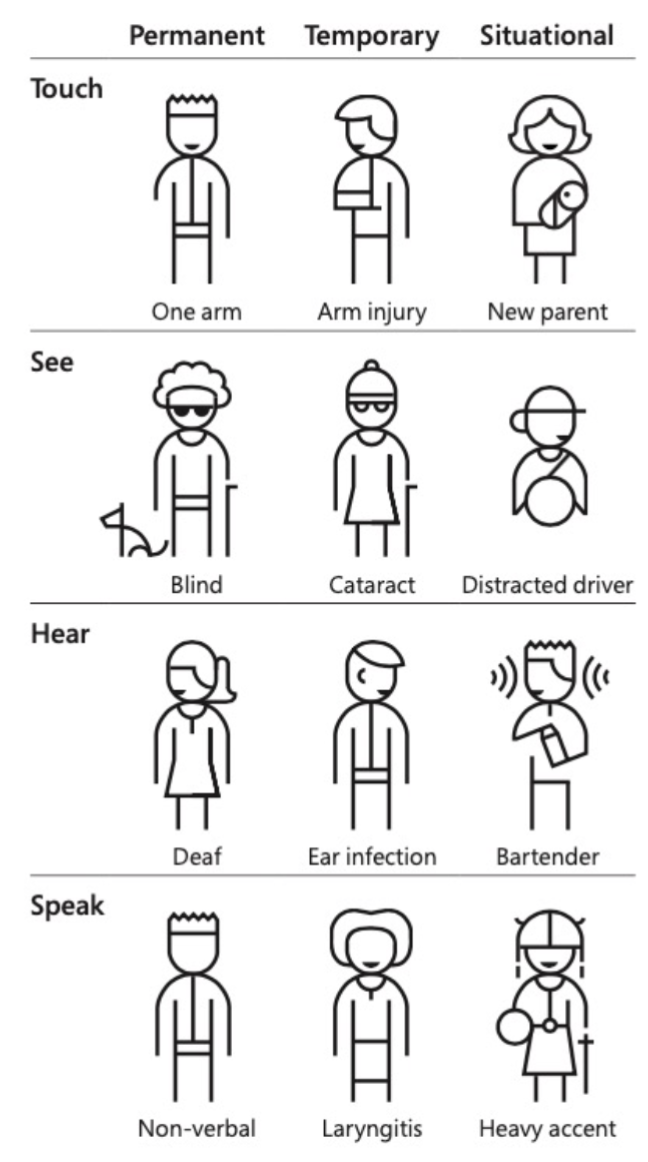
\includegraphics[scale=0.8]{lectures/wk13/img/disability_types.png}
\end{center}
Note that there are different types of Disabilities which have different extents. 

\begin{shaded}
Making sure audio can be heard for people who just are hard of hearing due to an ear infection and not only accommodating for people who are completely deaf is a necessity for accessible design.
\end{shaded}

\subsection{Solve for One, Extend to Many}
Curb Cuts (when the elevation in sidewalks goes down to meet the road) are helpful for people in wheelchairs, but are also helpful for new parents who have a baby in a stroller.

\subsubsection{Closed Captioning Usages:}
\begin{itemize}
    \item Started for deaf people
    \item Good for listening to accents
    \item Allows you to watch videos in public spaces where it's too loud to listen to audio
    \item Helpful for new language learners who do not know word pronunciations but know of the word in its spelling
\end{itemize}

\subsection{Specialized Hardware}
This can help with accessibility: Braille Display is an example of this (bumps on surfaces for blind people to feel what the display is saying).

\subsection{Visual: Screen Readers}
How do we make sure to not include the footer when reading a webpage out loud?\\
How do we `read' out loud images?
\begin{shaded}
    We can set the \texttt{alt} attribute of \texttt{<img>} tags to set what the image reads out loud. Note that this extends to give an alt text in case the image cannot load.
\end{shaded}

About 8 percent of men (one in 12) and 0.5 per cent of women (one in 200) have some form of red-green colour deficiency.

\subsubsection{Do not cause Seizures!}
Do not flash anything more than three times in a row.

\subsection{Navigable}
You can set the \texttt{tabindex} of \texttt{<div>} elements to set the sequential ordering that you navigate in when pressing the \texttt{Tab} key on your keyboard. 
